%======================================================================
% PoznQMI-4.pdf
%======================================================================
\section{Formalismus QM -- II}
\strana{QM-F-1}

Řekli jsme, že stavovým prostorem částice je $\mathcal{H} = L^2(\mathbb{R})$, tj.
\[
  \ket{\psi} = \int\psi(x')\ket{x'}\,\dd x' \qquad\dots\ \text{stav.\ prostor izomorf.\ s prost.\ } \forall\psi
\]
\[
  \|\psi\|^2 = \braket{\psi}{\psi} = \int\psi^*(x)\psi(x)\,\dd x < \infty
\]
Jak vypadají bázové vektory $\ket{x}$?

\subsection*{Diracova $\delta$-funkce}
\begin{minipage}{0.6\textwidth}
můžeme chápat jako limitu $\varepsilon\to 0$: \\
\dots\ částice lokalizovaná se stejnou amplitudou pravděpodobnosti v celém intervalu $\langle 0,\varepsilon\rangle$
\end{minipage}
\begin{minipage}{0.38\textwidth}
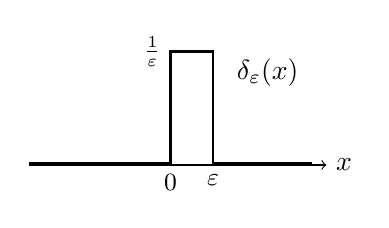
\begin{tikzpicture}[scale=0.9]
  \draw[->] (-2,0) -- (2.2,0) node[right] {$x$};
  \draw[thick] (-2,0.02) -- (0,0.02) -- (0,1.6) -- (0.6,1.6) -- (0.6,0.02) -- (2,0.02);
  \node[below] at (0,0) {\small $0$};
  \node[below] at (0.6,0) {\small $\varepsilon$};
  \node[left] at (0,1.6) {\small $\frac1\varepsilon$};
  \node[right] at (0.8,1.3) {$\delta_\varepsilon(x)$};
\end{tikzpicture}
\end{minipage}

\underline{problém:} \quad $\lim_{\varepsilon\to 0}\delta_\varepsilon(x)$ \ není dobře def.\ v $\mathcal{H}$

přesněji:
\begin{itemize}[nosep]
  \item[--] chápáno jako lim bod po bodu \dots\ $\delta_0 = 0$ skoro všude \quad ($\delta_0(0) = \infty$)
  \item[--] chápáno jako lim v $\mathcal{H}$ není Cauchy, neboť $\|\delta_\varepsilon\| = \sqrt{\varepsilon\cdot\frac{1}{\varepsilon^2}} = \frac{1}{\sqrt\varepsilon}\to\infty$
\end{itemize}

\begin{definice}[\uv{Rigged} Hilbertův prostor]
$\underline{\mathcal{H}}$ hustá podmn.\ v $\mathcal{H}$; \quad $\overline{\mathcal{H}} \equiv \underline{\mathcal{H}}^*$ \dots\ lin.\ spoj.\ funkcionály na $\underline{\mathcal{H}}$
\end{definice}

\textbf{PŘ:} \quad $\underline{\mathcal{H}} = \big\{\forall\psi(x)\in C^\infty(\mathbb{R});\ |\psi^{(n)}(x)(1+|x|)^m| < K\ \ \forall m,n\big\}$ \quad \kw{Schwartz space} \\
\quad v $\mathbb{R}^n$ obec.: $\sup|x^\alpha D^\beta f| < \infty$ $\forall\alpha,\beta$ \dots\ multiindexy

\textbf{PŘ:} \quad $\delta_\varepsilon(x)$ jako lin.\ funkcionál \quad $F_\varepsilon[\psi] = \int\delta_\varepsilon(x)\psi(x)\,\dd x$ \\
\quad opět $F_\varepsilon$ není limita v $\mathcal{H}^*$ \quad (nedefinuje spojitý funkcionál)

\begin{minipage}{0.65\textwidth}
\pozn{př: posl.\ fcí $\phi_n(x) = \frac{1}{1+e^{-nx}} \xrightarrow{n\to\infty} \Theta(x)$} \\
\pozn{přitom: $F_\varepsilon[\phi_n] \to \frac12$ \ ($\varepsilon\to 0$, fixní $n$)} \\
\pozn{ale \quad $F_\varepsilon[\phi_\infty] = 1$ \quad $\forall\varepsilon > 0$}
\end{minipage}
\begin{minipage}{0.33\textwidth}
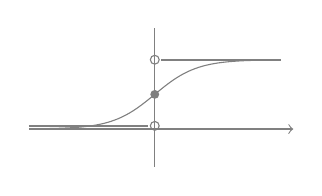
\begin{tikzpicture}[gray,scale=0.8]
  \draw[->] (-2,0) -- (2.2,0);
  \draw (0,-0.6) -- (0,1.6);
  \draw[thick] (-2,0.05) -- (-0.1,0.05);
  \draw (0,0.05) circle (2pt);
  \draw[thick] (0.1,1.1) -- (2,1.1);
  \draw (0,1.1) circle (2pt);
  \fill (0,0.55) circle (2pt);
  \draw[thin,domain=-1.8:1.8,samples=60] plot (\x,{1.1/(1+exp(-3*\x))});
\end{tikzpicture}
\end{minipage}

\dots\ volba $\underline{\mathcal{H}}$ spojité funkce \quad $F_\varepsilon[\psi(x)] \to \delta[\psi(x)] = \psi(0)$

\begin{itemize}
  \item další důležitá fce, která není v $\mathcal{H}$: \quad $e^{ipx}$ \dots\ je v $\overline{\mathcal{H}}$, pokud volíme testovací fce dostatečně ubývající. \\
        většinou: \quad $\underline{\mathcal{H}}$ \dots\ $\forall$ fce z $C^\infty$ ubývající rychleji než $\forall$ mocnina $|x|^n$ v $\infty$ (i jejich derivace)
\end{itemize}
\dots\ funkce jako $\delta(x - x_0)$, $e^{ikx}$, $\sin kx$ můžeme zahrnout jako prvky $\overline{\mathcal{H}}$

\textbf{Jiný příklad:} \quad $\ell^2 = \mathcal{H}$; \quad $\underline{\mathcal{H}} = \forall$ posl.\ $c_n$: $\sum_n|c_n|^2n^m < \infty$ \ $\forall m = 0,1,2,\dots$ \\
\quad potom $\overline{\mathcal{H}}$ lze složit \dots\ prostor $\forall v_n$: \ $\sum_n v_n^*c_n < \infty$ \ $\forall c_n\in\underline{\mathcal{H}}$

%----------------------------------------------------------------------
\strana{QM-F-2}
\subsection*{Další důležité příklady $\delta$-limit}
\begin{minipage}{0.68\textwidth}
\begin{itemize}[nosep]
  \item $\delta_\alpha(x) = \dfrac1\pi\dfrac{\alpha}{x^2+\alpha^2} \xrightarrow{\ \alpha\to 0\ } \delta(x)$ \quad \pozn{Lorentz}
  \item $\delta_\alpha(x) = \dfrac{\alpha}{\sqrt\pi}e^{-\alpha^2x^2} \xrightarrow{\ \alpha\to\infty\ } \delta(x)$ \quad \pozn{Gauss}
\end{itemize}
důležitý případ: \quad $\delta_\alpha(x) = \dfrac{\sin\alpha x}{\pi x} \xrightarrow{\ \alpha\to\infty\ } \delta(x)$ \dots
\end{minipage}
\begin{minipage}{0.3\textwidth}
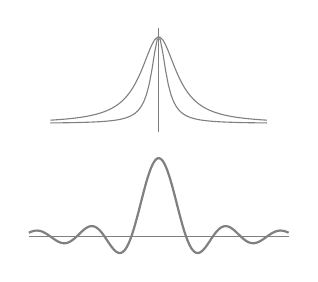
\begin{tikzpicture}[gray,scale=0.55]
  \draw[thin] (0,-0.2) -- (0,2.2);
  \draw[domain=-2.5:2.5,samples=80] plot (\x,{2*0.5^2/(\x*\x+0.5^2)});
  \draw[domain=-2.5:2.5,samples=80] plot (\x,{2*0.2^2/(\x*\x+0.2^2)});
  \begin{scope}[yshift=-2.6cm]
    \draw[thin] (-3,0) -- (3,0);
    \draw[thick,domain=-3:3,samples=150] plot (\x,{(abs(\x)<0.001) ? 1.8 : 1.8*sin(5*\x r)/(5*\x)});
  \end{scope}
\end{tikzpicture}
\end{minipage}

\dots\ základ Fourier.\ transformace:
\[
  \int e^{ikx}\,\dd k \ \longrightarrow\ \int_{-\alpha}^{\alpha}e^{ikx}\,\dd k = \frac{e^{i\alpha x} - e^{-i\alpha x}}{ix} = \frac{2\sin\alpha x}{x} \xrightarrow{\ \alpha\to\infty\ } 2\pi\delta(x)
\]
\noindent\rule{\linewidth}{0.3pt}
neboli \quad $\vzorec{\displaystyle\int e^{2\pi ikx}\,\dd k = \delta(x)}$

\begin{minipage}{0.6\textwidth}
užitečný vztah: \quad $\delta(x) = \Theta'(x)$ \quad \dots\ \pozn{$\lim_{\alpha\to 0}$}
\end{minipage}
\begin{minipage}{0.38\textwidth}
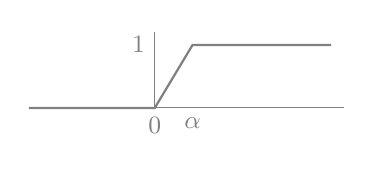
\begin{tikzpicture}[gray,scale=0.8]
  \draw (-2,0) -- (3,0);
  \draw (0,0) -- (0,1.2);
  \node[left] at (0,1) {\small $1$};
  \draw[thick] (-2,0) -- (0,0) -- (0.6,1) -- (2.8,1);
  \node[below] at (0,0) {\small $0$};
  \node[below] at (0.6,0) {\small $\alpha$};
\end{tikzpicture}
\end{minipage}

\noindent\rule{\linewidth}{0.3pt}

\subsection*{Použití $\delta(x)$ jako báze}
vztah \quad $\ket{\psi} = \int\psi(x')\ket{x'}\,\dd x'$ \quad \dots\ báze v $L^2$: \ $\ket{x'} = \delta(\xi - x')$
\[
  = \int\psi(x')\delta(\xi - x')\,\dd x' = \psi(\xi)\ \checkmark
\]
koef.\ rozvoje do báze: $\braket{n}{\psi} = \psi_n$ \quad \dots\ zde \quad
$\braket{x'}{\psi} = \int\delta(\xi - x')\psi(\xi)\,\dd\xi = \psi(x')\ \checkmark$

\pozor{pozor} \dots\ $\ket{x}$ nejde normovat konvenčním způsobem: \ \sout{$\braket{x}{x} = 1$} \\
místo toho \quad $\vzorec{\braket{x}{x'} = \int\dd\xi\,\delta(x - \xi)\delta(x' - \xi) = \delta(x - x')}$ \\
\quad \dots\ analogie \quad $\braket{n}{n'} = \delta_{nn'}$

Rozklad $\hat I$: \quad $I = \sum_n\ket{n}\bra{n}$ \quad \dots\ zde: \quad
$\begin{aligned}[t]\ket{x_0} &= \delta(x - x_0) \\ \bra{x_0} &= \delta(x - x_0)^* = \delta(x - x_0)\end{aligned}$
\[
  \text{tj.}\quad I = \int\dd x_0\ket{x_0}\bra{x_0} = \int\dd x_0\,\delta(\xi - x_0)\delta(\xi' - x_0) = \delta(\xi - \xi')
\]
\quad \dots\ zápis $I$ v $x$-reprezentaci \quad $\mel{x}{I}{x'} \equiv \braket{x}{x'} = \delta(x - x')$

zápis operátoru $Q$: \quad $Q\ket{x} = x\ket{x}$
\[
  \mel{x}{Q}{x'} = \int\dd\xi\,\delta(x - \xi)\,x'\,\delta(x' - \xi) = x'\delta(x - x') = x\,\delta(x - x')
\]

%----------------------------------------------------------------------
\strana{QM-F-3}
\subsection*{Více o operátorech}
$A:\ \mathcal{D}(A)\to\mathcal{R}(A)$; \quad $\overline{\mathcal{D}(A)} = \mathcal{H}$ \dots\ hustá množina \\
\quad $\mathcal{R}(A)\subset\mathcal{H}$ \dots\ obor hodnot. \quad \dots\ jinak nevíme dost dobře jak aplikovat na $\forall\ket{\psi}$

\begin{definice}[omezený operátor]
$\exists M:\ \dfrac{\|A\psi\|}{\|\psi\|} \leq M \quad \forall\psi\in\mathcal{D}(A)$ \\[2pt]
def: norma operátoru \quad $\|A\| = \sup_{\|\psi\|\leq 1}\|A\psi\|$
\end{definice}

\underline{pozn:} spojitost \dots\ v $\infty$ dim \dots\ $\forall$ lin.\ oper.\ je spojitý \\
\quad v $\mathcal{H}$: \ lin.\ operátor je spoj.\ $\Leftrightarrow$ omezený

\textbf{PŘ:}
\begin{itemize}[nosep]
  \item unitární operátor \quad $\|U\| = 1$ \quad protože $\|U\psi\| = \|\psi\|$
  \item $P$ \dots\ projektor \quad $\|P\|\leq 1$ \quad neboť
  \[
    \|P\psi\|^2 = \braket{P\psi}{P\psi} = |\braket{\psi}{P\psi}| \overset{\text{Schwarz}}{\leq} \|\psi\|\cdot\|P\psi\| \qquad\text{tj.}\quad \frac{\|P\psi\|}{\|\psi\|}\leq 1
  \]
\end{itemize}

\underline{Pozn:} díky spojitosti lze omez.\ oper.\ dodef.\ (rozšířit) na $\mathcal{H} = \overline{\mathcal{D}(A)}$ \\
\quad \dots\ úplnost \dots\ $\forall$ Cauchy $\psi_n\to\psi$ \dots\ $A\psi_n$ je rovněž Cauchy $\to\exists A\psi$

\textbf{PŘ:} F.T. \quad $\int f(x)e^{2\pi ikx}\,\dd x$ \dots\ je def.\ na $L_1$ nebo na $\mathcal{S}$ + rozšíření \\
\quad $\equiv F[f]$ \quad \dots\ $\|F\| = 1$

\pozor{Problém:} v QM se často setkáváme s neomez.\ operátory: \\
\quad $\exists\psi_n\in\mathcal{H}:\ \|\psi_n\| = 1:\ \|A\psi_n\|\to\infty$ \quad a \quad $\mathcal{D}(A)\subset\mathcal{H}$

\begin{priklad}[PŘ]
$\hat x\psi(x) = x\psi(x)$ \quad \dots\ $\mathcal{D}(A) = \big\{\psi(x)\in\mathcal{H};\ \int x^2|\psi|^2\dd x < \infty\big\}$

není omez.: \quad $\psi_n(x) = $
\tikz[baseline=2pt,scale=0.55]{
  \draw[->] (0,0) -- (4.2,0);
  \draw (0,0) -- (0,1.1);
  \node[left] at (0,1) {\scriptsize 1};
  \draw[dotted] (0,1) -- (2.5,1);
  \draw[thick] (2.5,0) -- (2.5,1) -- (3.3,1) -- (3.3,0);
  \node[below] at (2.5,0) {\scriptsize $n$};
  \node[below] at (3.4,0) {\scriptsize $n{+}1$};
}
\quad $\|\hat x\psi_n\|^2 = \int_n^{n+1}x^2\,\dd x = \frac13(3n^2 + 3n + 1)\to\infty$

podobně: \quad $\hat p = -i\hbar\dv{x}$ \quad \dots\ $\psi_n = N_ne^{inx}$ \quad \dots\ $\|\hat p\psi_n\| = \hbar n\|\psi_n\|\to\infty$
\end{priklad}

\dots\ Rigged spaces: \ $\underline{\mathcal{H}}\equiv\mathcal{D}$ \dots\ vl.\ vektory v $\overline{\mathcal{H}}$ \dots\ $\delta(x - \xi)$; $e^{\frac{i}{\hbar}p\xi}$ \\
\quad nebo nahrazení spektrálního rozkladu projektorovou mírou \dots

MATEMATICKÉ FOUSY \dots\ KOPÁČEK

%----------------------------------------------------------------------
\strana{QM-F-4}
\subsection*{Spektrum lineárního operátoru}
\underline{v $\not\infty$ dim:} \quad $A\ket{\phi} = \lambda\ket{\phi} \Leftrightarrow |A - \lambda I| = 0$ \\
\quad $\{\forall\lambda\}$ = spektrum (diskrétní) \dots\ spekt.\ rozklad \quad $A = \sum_\lambda\lambda P_\lambda$, \quad
$P_\lambda = \sum_{\ket{\phi}\text{ pro fix }\lambda}\ket{\phi}\bra{\phi}$

\underline{v $\infty$ dim:} \quad def.\ nemá smysl.

\sout{Matem.\ fousy: Symetrický $\times$ samosdružený operátor:}

\begin{definice}[spektrum lin.\ operátoru]
$\lambda\in\mathbb{C}$ nazveme \kw{bodem spektra} $\lambda\in\sigma(A)$, pokud $(A - \lambda I)$ není prosté a $\mathcal{H}$ na $\mathcal{H}$.
\end{definice}

Možnosti:
\begin{itemize}[nosep]
  \item[(i)] $(A - \lambda)$ není prosté, tj.\ $\exists\psi\neq 0:\ (A - \lambda)\psi = 0$. \\
             tj.\ $\psi\in\ker(A - \lambda)$ \quad \dots\ $\lambda\in\sigma_p(A)$ \dots\ \kw{bodové spektrum} \sout{(diskrétní)}
  \item[(ii)] $(A - \lambda)$ prosté, ale $\mathcal{R}(A - \lambda)\neq\mathcal{H}$
  \begin{itemize}[nosep]
    \item[a)] $\overline{\mathcal{R}(A - \lambda)} = \mathcal{H}$ \dots\ hustá v $\mathcal{H}$ \quad \dots\ $\lambda\in\sigma_c(A)$ \dots\ \kw{spojité spektrum}
    \item[b)] $\overline{\mathcal{R}(A - \lambda)}\neq\mathcal{H}$ \quad \dots\ $\lambda\in\sigma_R$ \dots\ \kw{reziduální spektrum}
  \end{itemize}
\end{itemize}
Zde se operátory s $\sigma_R$ zabývat nebudeme.

\begin{definice}[Normální operátor]
$[A, A^\dagger] = 0$ \quad pak \quad
$\lambda\in\sigma(A) \Leftrightarrow \exists\psi_n\in\mathcal{H},\ \|\psi_n\| = 1,\ \lim_{n\to\infty}(A - \lambda)\psi_n = 0$
\end{definice}

\begin{priklad}[PŘ: operátor $\hat x$]
\dots\ posloupnost \quad $\psi_n = \sqrt n\,\chi_{\langle x_0,x_0+\frac1n\rangle}$ \quad \dots\ $\|\psi_n\| = 1$ \\
neboť \quad $\|(\hat x - x_0)\psi_n\|^2 = \int_{x_0}^{x_0+\frac1n}(x - x_0)^2n\,\dd x = n\cdot\frac13\big(\frac1n\big)^3 = \frac13n^{-2}\to 0$ \\
ale $\psi_n$ není Cauchy (výše) \dots\ má však limitu v $\overline{\mathcal{H}}$ $\to\delta(x - x_0)$ \\
(po přenormování \dots\ norma na $\overline{\mathcal{H}}$ je jiná než na $\mathcal{H}$)
\end{priklad}

\begin{itemize}
  \item více o \underline{normálních operátorech}: \hfill \dots\ spec.\ př.\ \dots\ $A = A^\dagger$; $U^\dagger = U^{-1}$
\end{itemize}
\underline{v $\not\infty$ dim:}
\begin{enumerate}[label=\arabic*),nosep]
  \item $A\ket{\psi} = \lambda\ket{\psi} \Rightarrow A^\dagger\ket{\psi} = \lambda^*\ket{\psi}$ \hfill \dots\ unit.\ $\lambda^* = \lambda^{-1}$ \dots\ $|\lambda| = 1$
  \item $\lambda_1\neq\lambda_2$ vl.\ č.\ $\Rightarrow\ \braket{\psi_1}{\psi_2} = 0$
  \item vl.\ v.\ tvoří ON bázi
\end{enumerate}
důvod: každý operátor mohu rozložit: \quad $A = \dfrac{A + A^\dagger}{2} + i\dfrac{A - A^\dagger}{2i} = C + iD$, \\
\quad kde $C, D$ hermitovské, navíc $[A, A^\dagger] = 0 \Rightarrow [C, D] = 0$ \\
\quad tj.\ mají spol.\ bázi vl.\ v.

Normální operátor \dots\ komplex.\ zobecnění reál.\ Hermit.\ operátoru

%----------------------------------------------------------------------
\strana{QM-F-5}
\providecommand{\sumint}{\mathop{\textstyle\sum\hspace{-1.05em}\int}}
\subsection*{Další matematické fousy}
\underline{Symetrický $\times$ Samosdružený operátor:}

\begin{definice}
\kw{symetrický} (Hermitovský): \quad $(A\phi,\psi) = (\phi,A\psi)\quad\forall\phi,\psi\in\mathcal{D}(A)$ \\
\kw{samosdružený} \dots\ navíc \quad $\mathcal{D}(A) = \mathcal{D}(A^\dagger)$
\end{definice}
(pozn: relace $(\psi,A\phi) = (A^\dagger\psi,\phi)$ může definovat $A^\dagger\ket{\psi}$ i pro $\psi$ mimo $\mathcal{D}(A)$)

\pozor{pojem samosdruženosti podstatně závisí na prostoru na němž def.\ $A$!} \ (a spektra)

\begin{priklad}[Př: $P = -i\dv{x}$ \dots\ neomezený, symetrický (v záv.\ na prostoru)]
\begin{align*}
  \mel{\phi}{D^\dagger}{\psi} \equiv \braket{D\phi}{\psi} &= i\int_a^b\phi^{*\prime}(x)\psi(x)\,\dd x = \text{(per partes)} \\
  &= i\big[\psi(x)\phi^*(x)\big]_a^b - i\int\phi^*(x)\psi'(x)\,\dd x = [\ \ ] + \mel{\phi}{D}{\psi}
\end{align*}
tj.\ závisí na okraj.\ podm.: \hfill $Pe^{i\lambda x} = \lambda e^{i\lambda x}$
\begin{itemize}[nosep]
  \item[(a)] fce na $(-\infty,\infty)$ bez podm.: $P$ není sym., $\forall\lambda\in\mathbb{C}$ je vl.\ č.
  \item[(b)] fce omezené pro $|x|\to\infty$: $P$ nesym.; $\lambda\in\mathbb{R}$ jsou vl.\ č.
  \item[(c)] na $\langle 0,L\rangle$ period.\ fce: $P$ symetrický, \ $\lambda = \lambda_n = \frac{2\pi n}{L}$, $n\in\mathbb{Z}$ vl.\ č.
  \item[(d)] fce na $(-\infty,\infty)$; $|\phi|\to 0$ pro $|x|\to\infty$: $P$ symetrický, ale nemá vl.\ fce.
\end{itemize}
\end{priklad}

\begin{veta}[Samosdružený operátor]
má úplnou množinu (zobecněných) vlastních funkcí: \\
Spektrální rozklad: \quad $I = \int P_a\,\dd a + \sum_n P_n$ \quad $\leftarrow$ \kw{úplnost}
\[
  \vzorec{A = \int aP_a\,\dd a + \sum_n a_nP_n} \quad \pozn{$= \sumint_{a\in\sigma(A)} aP_a$}
\]
\end{veta}
v případě nedegener.\ spektra: \quad $P_n = \ket{a_n}\bra{a_n}$, \quad $P_a = \ket{a}\bra{a}$ \\
\phantom{v případě} degenerované: \quad $P_n = \sumint_\alpha\ket{a_n,\alpha}\bra{a_n,\alpha}$, \quad $P_nP_{n'} = P_n\delta_{nn'}$ \\
\phantom{v případě degenerované:} \quad $P_a = \sumint_\alpha\ket{a,\alpha}\bra{a,\alpha}$, \quad $P_aP_{a'} = P_a\delta(a - a')$ \quad $\leftarrow$ \underline{ortogonalita}

\begin{priklad}[PŘ: v $\mathcal{H} = L^2(\mathbb{R}^3)$ operátor $Q_1\equiv\hat x_1$]
\[
  \hat x_1 = \int\dd x_1\,x_1P_{x_1};\quad\text{kde}\quad P_{x_1} = \int\dd x_2\dd x_3\ket{x_1x_2x_3}\bra{x_1x_2x_3}
  \quad\text{tj.}\ = \int\dd x_2\dd x_3\ket{\vec x}\bra{\vec x}
\]
nebo \quad $\hat x_1 = \int\dd^3x\,x_1\ket{\vec x}\bra{\vec x}$
\end{priklad}
Příklady operátorů se spojitým i diskr.\ spektrem uvidíme později (H pro systém s vázanými stavy)

\underline{pozn:} \quad $f(\hat A) = \sumint_a f(a)\hat P_a$ \qquad
\underline{pozn:} samosdr.\ $\hat A$ omezený $\Leftrightarrow\sigma(\hat A)$ omez. \quad $\|\hat A\| = \sup\sigma(\hat A)$

%----------------------------------------------------------------------
\strana{QM-F-6}
matematické fousy? \ co je $\ket{x}\bra{x}$ za objekt? \\
$\to$ my budeme pracovat intuitivně \dots\ např.\ $\ket{x}\braket{x}{\psi} = \psi(x)\cdot\ket{x}$ \\
podrobněji:

\begin{veta}[Spektrální teorém]
$\forall$ samosdružený operátor $A$ $\exists$ funkce $E(\lambda)$; kde $\lambda\in\mathbb{R}$ a $E$ je projekční operátor na $\mathcal{H}$ taková, že:
\begin{enumerate}[label=\arabic*),nosep]
  \item $\forall\lambda_1 < \lambda_2$: \quad $E(\lambda_1)E(\lambda_2) = E(\lambda_2)E(\lambda_1) = E(\lambda_1)$
  \item $\forall\ket{\psi}$: \quad $E(\lambda+\varepsilon)\ket{\psi}\to E(\lambda)\ket{\psi}$, \quad $\varepsilon\to 0^+$
  \item \phantom{$\forall\ket{\psi}$:} \quad $E(\lambda)\ket{\psi}\to 0$; \quad $\lambda\to -\infty$
  \item \phantom{$\forall\ket{\psi}$:} \quad $E(\lambda)\ket{\psi}\to\ket{\psi}$; \quad $\lambda\to +\infty$
  \item $\int\lambda\,\dd E(\lambda) = A$
\end{enumerate}
\end{veta}
kde $\int f(\lambda)\,\dd E(\lambda)$ je definovaný jako (Stieltjesův integrál):
\[
  \int f(\lambda)\,\dd E(\lambda) \equiv \lim_{\substack{n\to\infty\\ \Delta\lambda\to 0}}\sum_{k=1}^{\infty\,(n)} f(\lambda_k)\big[E(\lambda_k) - E(\lambda_{k-1})\big]
\]

\underline{poznámka:}
\begin{itemize}
  \item Tato formulace je trik, jak napsat předchozí formulaci v $\overline{\mathcal{H}}$ do $\mathcal{H}$. Přičemž
  \[ E(\lambda) = \sum_{a_n<\lambda}P_n + \int_{a<\lambda}P_a\,\dd a \qquad (*) \]
  $\to$ ověřte, že $(*)$ splňuje 1)--5)
\end{itemize}

Ad 5):
\begin{center}
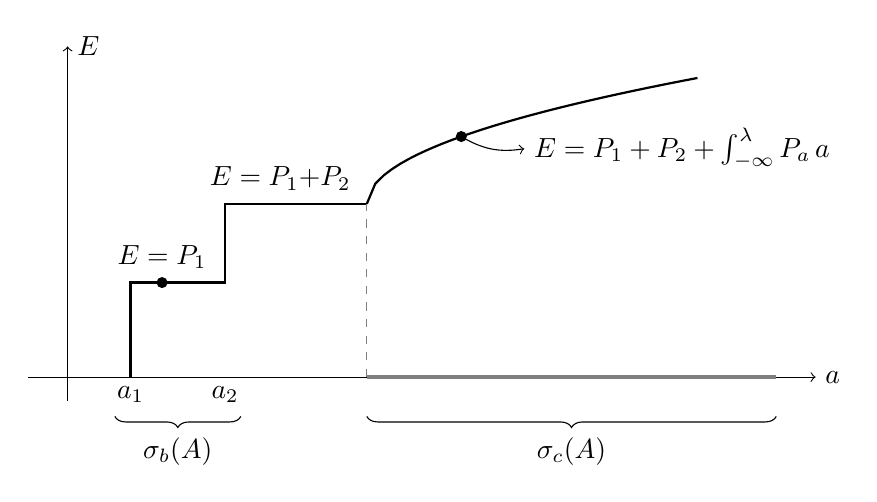
\begin{tikzpicture}[x=1cm,y=1cm]
  \draw[->] (-0.5,0) -- (9.5,0) node[right] {$a$};
  \draw[->] (0,-0.3) -- (0,4.2) node[right] {$E$};
  \draw[thick] (0.8,0) -- (0.8,1.2) -- (2,1.2) -- (2,2.2) -- (3.8,2.2);
  \fill (1.2,1.2) circle (2pt);
  \node[above] at (1.2,1.25) {$E = P_1$};
  \node[above] at (2.7,2.25) {$E = P_1{+}P_2$};
  \draw[thick,domain=3.8:8,samples=40] plot (\x,{2.2 + 0.6*sqrt(\x-3.8)*1.3});
  \fill (5,{2.2+0.6*sqrt(1.2)*1.3}) circle (2pt);
  \draw[->] (5,{2.2+0.6*sqrt(1.2)*1.3}) to[bend right=20] (5.8,2.9) node[right] {$E = P_1 + P_2 + \int_{-\infty}^{\lambda}P_a\,\dd a$};
  \draw[ultra thick,gray] (3.8,0) -- (9,0);
  \draw[dashed,gray] (3.8,0) -- (3.8,2.2);
  \node[below] at (0.8,0) {$a_1$};
  \node[below] at (2,0) {$a_2$};
  \draw[decorate,decoration={brace,mirror,amplitude=4pt}] (0.6,-0.5) -- (2.2,-0.5) node[midway,below=4pt] {$\sigma_b(A)$};
  \draw[decorate,decoration={brace,mirror,amplitude=4pt}] (3.8,-0.5) -- (9,-0.5) node[midway,below=4pt] {$\sigma_c(A)$};
\end{tikzpicture}
\end{center}

tj.\ pro spojité spektrum:
\[
  \int\lambda\,\dd E(\lambda) \equiv \sum_{k=1}^{\infty}\underbrace{f(\lambda_k)}_{\lambda_k}\underbrace{\big[E(\lambda_k) - E(\lambda_{k-1})\big]}_{\Delta\lambda_k\to 0\ \dots\ E\text{ spojité: }\Delta E\doteq\frac{\dd E}{\dd\lambda}\cdot\Delta\lambda}
  = \sum\lambda_k\frac{\dd E}{\dd\lambda}(\lambda_k)\cdot\Delta\lambda
\]
\[
  \xrightarrow{\ \Delta\lambda\to 0\ } \int\lambda\frac{\dd E(\lambda)}{\dd\lambda}\,\dd\lambda = \int\lambda P_\lambda\,\dd\lambda
  \qquad\text{neboť}\quad \dv{\lambda}\int_{-\infty}^{\lambda}P_a\,\dd a = P_\lambda
  \quad\text{tj.}\quad \vzorec{\frac{\dd E(\lambda)}{\dd\lambda} = P_\lambda}
\]
ale $E(\lambda)$ má smysl i $\mathcal{H}$; \ $P_\lambda$ jen v $\overline{\mathcal{H}}$

%----------------------------------------------------------------------
\strana{QM-F-7}
\underline{diskrétní spektrum:} \\
stačí si uvědomit, že $E(\lambda_k) - E(\lambda_{k-1})\neq 0$ jen v okolí bodů spektra a tam je
$E(\lambda_k) - E(\lambda_{k-1}) = P_n$ \quad \dots\ $\lambda_k\geq a_n > \lambda_{k-1}$ \\
tj.: \quad $\int\lambda\,\dd E(\lambda) = \sum_n a_nP_n$
\begin{itemize}
  \item lze také chápat jako $E(\lambda) = \sum_n\Theta(\lambda - a_n)P_n$, potom:
  \[
    \int\lambda\,\dd E(\lambda) = \int\lambda\frac{\dd E}{\dd\lambda}\cdot\dd\lambda
    = \int\lambda\sum_n\underbrace{\dv{\lambda}\Theta(\lambda - a_n)}_{\delta(\lambda - a_n)}P_n\,\dd\lambda = \sum_n a_nP_n
  \]
\end{itemize}
\noindent\rule{\linewidth}{0.3pt}

\subsection*{Doplnění k axiomům QM}
\begin{veta}[Axiomy QM]
\begin{itemize}[nosep]
  \item[\fbox{A1}] Stav systému je dán paprskem v $\mathcal{H}$.
  \item[\fbox{A2}] Každé dynamické proměnné (měřitelné veličině, pozorovatelné) odpovídá samosdružený lineární operátor, jehož spektrum udává možné výsledky měření.
  \item[\fbox{A3}] Výsledky měření předpovídáme pomocí spektrálního rozkladu operátoru: \\
  hustota pravděpodobnosti nalezení hodnoty $a$ ve stavu $\ket{\psi}$
  \[
    \mu_\psi(a)\,\dd a = \mel{\psi}{\hat P(a)}{\psi}\,\dd a \qquad \big(= \mel{\psi}{\dd E(a)}{\psi}\big)
  \]
  pravděpodobnost nalezení hodnoty $a\in\mathcal{M}$:
  \[
    \mu = \int_{\mathcal{M}}\mu_\psi(a)\,\dd a
  \]
  stav po měření: \quad $\ket{\psi'} = \int_{\mathcal{M}}P(a)\ket{\psi}\,\dd a$ \quad $\big(= \int_{\mathcal{M}}\dd E(a)\ket{\psi}\big)$
\end{itemize}
\end{veta}

\underline{pozn:}
\begin{itemize}[nosep]
  \item[--] dále platí \quad $\mu = \braket{\psi'}{\psi'} \equiv \|\psi'\|^2$ \quad
            \pozn{\dots\ $\braket{\psi'}{\psi'} = \int_{\mathcal{M}}\int_{\mathcal{M}}\mel{\psi}{\underbrace{P(a')P(a)}_{\delta(a,a')I}}{\psi}\,\dd a\,\dd a'$}
  \item[--] $\mu$ nalezení vůbec nějaké hodn.\ $= 1 = \int_{\mathbb{R}}\mu_\psi(a)\,\dd a = \mel{\psi}{\hat I}{\psi}$ \quad \pozn{$\hat I = \int_{\mathbb{R}}P_a\,\dd a$}
\end{itemize}

\begin{priklad}[PŘ: Pravděpodobnost nalezení částice v místě $x\in\langle a,b\rangle$ (1D)]
\dots\ částice ve stavu $\ket{\psi} = \int\psi(x)\ket{x}\,\dd x$ \\
\dots\ měřitelná veličina \quad $\hat Q\equiv\hat x = \int\ket{x}\bra{x}\,\dd x$ \quad \dots\ spektr.\ rozklad $P_x = \ket{x}\bra{x}$
\[
  \text{tj.}\quad \mu_{\langle a,b\rangle} = \int_a^b\braket{\psi}{x}\braket{x}{\psi}\,\dd x = \int_a^b|\psi|^2\,\dd x
\]
po měření ve stavu \quad $\ket{\psi'} = \int_a^bP_x\ket{\psi}\,\dd x = \int_a^b\psi(x)\ket{x}\,\dd x$ \\
\phantom{po měření ve stavu} \quad tj.\ $\psi'(x) = \chi_{\langle a,b\rangle}(x)\psi(x)$
\end{priklad}
\underline{pozn:} \quad $\rho(x)\equiv|\psi(x)|^2$ \quad \dots\ \kw{hustota pravd.\ výskytu} částice v místě $x$

%----------------------------------------------------------------------
\strana{QM-F-8}
\subsection*{Další statistické veličiny}
z matematického hlediska měření $A$ ve stavu $\ket{\psi}$ \\
$\to$ náhodná proměnná: opakované měření dá pokaždé jinou hodnotu $a\in\sigma(A)$ s rozdělovací funkcí $\mu_\psi(a)$

střední hodnota náhod.\ prom.: \quad $\langle a\rangle \equiv \int a\,\mu_\psi(a)\,\dd a = \int a\mel{\psi}{P_a}{\psi}\,\dd a$
\[
  \text{tj.}\quad \vzorec{\langle a\rangle = \mel{\psi}{A}{\psi}} \qquad (\text{normované } \ket{\psi}!)
\]
vyšší momenty náhod.\ prom.: \quad $\langle a^n\rangle \equiv \int a^n\mu_\psi(a)\,\dd a = \mel{\psi}{A^n}{\psi}$ \\
obec.\ $\to$ fce náhod.\ prom. \quad $\langle f(a)\rangle \equiv \int f(a)\mu_\psi(a)\,\dd a = \mel{\psi}{f(A)}{\psi}$

důležitý případ \underline{variance} (střední kvadr.\ odchylka, rozptyl): \\
\quad značení $\sigma_a^2$ nebo \quad $(\Delta a)^2 \equiv \big\langle(a - \langle a\rangle)^2\big\rangle = \langle a^2\rangle - \langle a\rangle^2$

\underline{pozn:} ve vl.\ stavu: $A\ket{\psi} = a\ket{\psi}$ \quad \dots\
$\left.\begin{aligned}\langle A\rangle &= a\\ \langle A^2\rangle &= a^2\end{aligned}\right\}\to(\Delta A)^2 = 0$

\subsection*{Relace neurčitosti}
\begin{veta}[Relace neurčitosti]
nechť $[\hat A,\hat B] = i\hat C$ \quad potom \quad $\vzorec{\Delta a\cdot\Delta b \geq \tfrac12|\mel{\psi}{\hat C}{\psi}|}$
\end{veta}
\underline{pozn:} im.\ jednotka zaručuje: pokud $A = A^\dagger$, $B = B^\dagger\Rightarrow C = C^\dagger$

\underline{DK:} \quad Schwarzova nerovnost: \quad $\|\phi_1\|\cdot\|\phi_2\| \geq |\braket{\phi_1}{\phi_2}|$ \quad $(*)$ \\
\quad pro \quad $\ket{\phi_1} = (A - \langle a\rangle)\ket{\psi}$ \quad \dots\ $\|\phi_1\| = \sqrt{\mel{\psi}{(A - \langle a\rangle)^2}{\psi}} = \Delta a$ \\
\quad podob.\ \quad $\ket{\phi_2} = (B - \langle b\rangle)\ket{\psi}$ \quad \dots\ $\|\phi_2\| = \Delta b$ \\
pravá str.\ $(*)$:
\begin{align*}
  |\braket{\phi_1}{\phi_2}| &= |\mel{\psi}{(A - \langle a\rangle)(B - \langle b\rangle)}{\psi}| = |\mel{\psi}{AB - \langle a\rangle\langle b\rangle}{\psi}| \\
  &= \Big|\bra{\psi}\frac{AB - BA}{2} + \frac{AB + BA}{2} - \langle a\rangle\langle b\rangle\ket{\psi}\Big| \\
  &= \Big|\underbrace{\tfrac{i}{2}\mel{\psi}{C}{\psi}}_{\text{ryze imag}} + \underbrace{\bra{\psi}\tfrac{AB+BA}{2}\ket{\psi} - \langle a\rangle\langle b\rangle}_{\text{reálné}}\Big|
  \geq \tfrac12|\mel{\psi}{C}{\psi}| \qquad\text{c.b.d.}
\end{align*}

nejznámější příklad: \quad $[x_1,p_1] = i\hbar$ \quad $\to$ \quad $\vzorec{\Delta x\cdot\Delta p \geq \tfrac{\hbar}{2}}$

%----------------------------------------------------------------------
\strana{QM-F-9}
\subsection*{Kompatibilní pozorovatelné}
\begin{veta}
Pokud $[A,B] = 0$, pak vl.\ prostory $A$ jsou invariantní vůči $B$ a naopak:
\[ A\ket{\psi} = a\ket{\psi} \ \Rightarrow\ A\ket{\phi} = a\ket{\phi} \quad\text{kde}\quad \ket{\phi} = B\ket{\psi} \]
\end{veta}

\begin{veta}
Nechť $A, B$ jsou samosdružené operátory. \\
Potom existuje úplná množina společných vl.\ v.\ $\Leftrightarrow$ $[A,B] = 0$
\end{veta}

\underline{DK:} \hfill {\color{red}Dělal jsem jinak -- viz dodatek} \\
\quad ($\Rightarrow$) je triviální důsledek spektrálního rozkladu \\
\quad ($\Leftarrow$) konstruktivní dk \dots\ sada vektorů $P_b\ket{a_n}$ $\forall b, a_n$
\begin{itemize}[nosep]
  \item[\dots] některé mohou být nulové, ale je úplná: \quad $\ket{\psi} = \sum_n\psi_n\ket{a_n} = \sum_{nb}\psi_nP_b\ket{a_n}$
  \item[\dots] jsou vl.\ v.\ $B$ \dots\ $b$
  \item[\dots] jsou vl.\ v.\ $A$ \dots\ a) $(A - a_n)\hat P_b\ket{a_n}$ je také vl.\ v.\ $B$ přísl.\ $b$ \dots\ $\psi_{nb}$ \\
        neboť \quad $B(A - a_n)P_b\ket{a_n} = (A - a_n)BP_b\ket{a_n} = b(A - a_n)P_b\ket{a_n}$ \\
        b): \quad $(A - a_n)\ket{a_n} = \sum_b(A - a_n)P_b\ket{a_n} = 0 = \sum_b\psi_{nb}$ \\
        $\to$ jednotlivé členy sumy jsou OG (různé $b$) a tedy $\psi_{nb} = 0$ $\forall b, n$
\end{itemize}

\underline{pozn:} důsl.\ \quad $[A,B] = 0 \Leftrightarrow [P_a,P_b] = 0\quad\forall a,b$ \\
\quad \pozn{DK: $\Leftarrow$ spektr.\ rozklad; $\Rightarrow$ rozepíšu $P_a, P_b$ pomocí spol.\ báze}

\underline{pozn:} některé $P_b\ket{a_n}$ mohli být nulové $\to$ množina $\forall\ket{ba_n}$ nemusí být kartézský součin \dots\ později např.\ $\ket{\ell m}$

+ Rozšíření na více operátorů
\subsection*{Úplný systém komutujících operátorů (ÚSKO)}
$\hat A^{(1)},\dots,\hat A^{(N)}$ navzájem komutují $\Rightarrow$ $\exists$ spol.\ báze vl.\ v.\ $\forall$ operátorů

\begin{definice}[ÚSKO]
$\forall$ sada vl.\ č.\ $\{a^{(1)},\dots,a^{(N)}\}$ (každá přípustná) jednoznačně def.\ vl.\ v.\ $\ket{\psi}$ (až na fázi) \\
\dots\ \underline{značení} \quad $\ket{\psi} = \ket{a^{(1)}\dots a^{(N)}}$
\end{definice}

\begin{veta}
operátor $\hat F$ komutuje se $\forall A^{(1)},\dots,A^{(N)}$ prvky ÚSKO $\Rightarrow$ $\hat F = f(A^{(1)},\dots,A^{(N)})$
\end{veta}
\underline{DK:} $\hat F, A^{(1)},\dots,A^{(N)}$ mají spol.\ sadu vl.\ v., ale to musí být $\ket{a^{(1)}\dots a^{(N)}}$ \\
\quad spektr.\ rozklad $\hat F$ $\to$ $\forall a^{(1)},\dots,a^{(N)}$ $\exists$ jediné $f = f(a^{(1)},\dots,a^{(N)})$

\underline{pozn:} celou množinu $\hat A^{(1)},\dots,\hat A^{(N)}$ lze považovat za jeden oper.\ s nedegenerovaným spektrem \dots\ vl.\ č.\ vektor

\textbf{PŘ:} \quad $Q_1, Q_2, Q_3$ \quad $\to$ spol.\ báze $\ket{\vec x}$

%----------------------------------------------------------------------
\strana{QM-F-10}
\begin{priklad}[typický příklad]
$\mathcal{H} = \mathcal{H}^{(A)}\otimes\mathcal{H}^{(B)}$; \quad
$\begin{aligned}[t] &A^{(1)}\dots A^{(N)} \ \dots\ \text{ÚSKO NA } \mathcal{H}^{(A)} \\ &B^{(1)}\dots B^{(M)} \ \dots\ \text{ÚSKO NA } \mathcal{H}^{(B)}\end{aligned}$

potom \quad $A^{(1)}\otimes I,\dots,A^{(N)}\otimes I,\ I\otimes B^{(1)},\dots,I\otimes B^{(M)}$ \ je ÚSKO na $\mathcal{H}$
\end{priklad}
\underline{pozn:} operátor $C = A + B$ \dots\ diagonalizovat \dots\ $[A,B] = 0 \Leftrightarrow$ najít spol.\ bázi $\to$ častý případ v QM

\subsection*{Různé ekvivalentní reprezentace QM}
\begin{itemize}
  \item \underline{volba ÚSKO} $\to$ báze + vyjádření vln.\ fce a oper.\ v bázi
\end{itemize}
\begin{itemize}[nosep]
  \item[--] diskrétní případ: \quad $I = \sum_n\ket{n}\bra{n}$ \quad \dots\ stavy \quad
  $\ket{\psi} = \sum_n\ket{n}\underbrace{\braket{n}{\psi}}_{\psi_n} \equiv \ket{\psi}$ \quad (izomorfizm.) ztotožnění \\
  operátory \quad $A\ket{\psi} = \sum_{nn'}\ket{n}\underbrace{\mel{n}{A}{n'}\braket{n'}{\psi}}_{A_{nn'}\psi_{n'}}$ \quad \dots\ $A\equiv A_{nn'}$
  \item[--] spojitý případ: \quad $I = \int\ket{\nu}\bra{\nu}\,\dd\nu$ \quad
  $\ket{\psi} = \int\dd\nu\,\psi(\nu)\ket{\nu}$ \quad ($\braket{\nu}{\psi} \equiv \ket{\psi}$)
  \[
    A\ket{\psi} = \int\dd\nu\,\dd\nu'\ket{\nu}\underbrace{\mel{\nu}{A}{\nu'}}_{A_{\nu\nu'}\equiv A(\nu,\nu')}\braket{\nu'}{\psi}
    \quad\dots\ \text{jádro integrálního operátoru}
  \]
\end{itemize}

\begin{priklad}[PŘ]
\begin{tabular}{lll}
$\hat x$ & $\leftrightarrow\ x\,\delta(x - x')$ & \dots\ $\int\dd x'\,x\,\delta(x - x')\psi(x') = x\psi(x)$ \\[2pt]
$V(\hat x)$ & $\phantom{\leftrightarrow}\ V(x)\delta(x - x')$ & $A\ket{\psi}$ \dots\ $V(x)\psi(x)$ \\[2pt]
$\hat p$ & $\leftrightarrow\ {-i\hbar}\,\delta'(x - x')$ & $= \int\dd x'\,i\hbar\,\delta'(x - x')\psi(x')\,\dd x' = -i\hbar\dv{x}\psi(x)$
\end{tabular}

\quad $\uparrow$ jiný zápis $-i\hbar\,\delta(x - x')\dv{x'}$

\pozn{podrobněji \ $-i\hbar\,\delta'(x - x') \equiv -i\hbar\dv{x}\delta(x - x') = +i\hbar\dv{x'}\delta(x - x')$ + per partes}
\end{priklad}

%----------------------------------------------------------------------
\strana{QM-F-11}
\subsection*{DODATEK}
\pozn{celá strana psána tužkou}


\textbf{Lemma 1:} \quad $[A,B] = 0\ \wedge\ B\ket{\psi} = b\ket{\psi}$ \quad $\Rightarrow$ \quad $B\ket{\phi} = b\ket{\phi}$; kde $\ket{\phi} = A\ket{\psi}$ \\
\quad DK: zjevné

\textbf{Lemma 2:} \quad $[A,B] = 0$, \ $a_1\neq a_2$ \quad $\Rightarrow$ \quad $\mel{a_1}{B}{a_2} = 0$ \\
\quad DK: \quad $0 = \mel{a_1}{[A,B]}{a_2} = \mel{a_1}{AB}{a_2} - \mel{a_1}{BA}{a_2}$ \\
\quad\phantom{DK:} tj. \ $0 = (a_1 - a_2)\mel{a_1}{B}{a_2}$ \quad $\Rightarrow$ c.b.d.

\textbf{Lemma 3a:} \quad $[A,B] = 0$ \quad $\Rightarrow$ \quad $[P_a,B] = 0$ \\
\quad DK: \ v bázi vl.\ v.\ $A$: \quad $A\ket{a,\alpha} = a\ket{a,\alpha}$ $\to$ $P_a = \sum_\alpha\ket{a\alpha}\bra{a\alpha}$
\begin{align*}
  \mel{a_1\alpha_1}{[P_a,B]}{a_2\alpha_2} &= \bra{a_1\alpha_1}\sum_\alpha\ket{a\alpha}\bra{a\alpha}B\ket{a_2\alpha_2}
   - \underbrace{\bra{a_1\alpha_1}B\sum_\alpha\ket{a\alpha}}_{\delta_{a_1a}\mel{a}{B}{a}}\underbrace{\braket{a\alpha}{a_2\alpha_2}}_{\delta_{aa_2}\delta_{\alpha\alpha_2}} \\
  \text{podle lemm.\ 1, 2!}\qquad &= \delta_{aa_1}\delta_{aa_2}\big\{\mel{a\alpha_1}{B}{a\alpha_2} - \mel{a\alpha_1}{B}{a\alpha_2}\big\} \\
  &= 0
\end{align*}

\textbf{Lemma 3:} \quad $[A,B] = 0$ \quad $\Rightarrow$ \quad $[P_a,P_b] = 0\quad\forall a,b$ \\
\quad DK: uplatnění lemm.\ 3a na $[P_a,B]$

$\Rightarrow$ $\exists$ společná báze \dots\ projektory $P_aP_b = P_bP_a$

